\documentclass{article}
\usepackage[utf8]{inputenc}
\usepackage{amsmath}
\usepackage{amssymb}
\usepackage{xcolor}
\usepackage{comment}
\DeclareMathOperator*{\argmax}{arg\,max}
\usepackage[margin=1.2in]{geometry}
\usepackage{graphicx}
\usepackage{algorithm}
\usepackage{algorithmic}
\usepackage{comment}

\title{Hidden Markov Models in Bioinformatics}
\author{Alexander J Ohrt - UPC BarcelonaTech}
\date{\today}

\begin{document}

\maketitle

\tableofcontents

\section{Introduction}
\textcolor{red}{These two first parts should be reviewed (perhaps written when done with the rest of the report)}
This report will present the uses of Hidden Markov Models (HMMs) in Bioinformatics. It will explain and highlight why they are populaar alternative tools for solving a wide range of problems in the field. In order to understand why HMMs are useful, and why they can be used effectively, some background on stochastic processses and Markov Chains is needed. Moreover, for completeness, a brief theoretical construct of some different HMMs will be done. In the remaining part of the report, a range of problems in Bioinformatics will be presented, first solved without the use of HMMs, then contrasted with the HMM based solutions. This will hopefully highlight why HMMs are effective alternatives. Note that this report is by no means extensive; there exists a plethora of theory and problems where the HMMs can be used. 

\section{Objectives}

The main objective of this report is to explain why HMMs are very widely used in Bioinformatics. Several problems in the field of study will be presented, with common solutions. First of all, solutions that are not based on HMMs will be shown, with their strengths and weaknesses. These will be contrasted with solution based on HMMs, which in all cases yield alternative methods which oftentimes perform better in some respect. For completeness, the reader should get a quick introduction to the vast theoretical background for HMMs, which includes a quick look at Markov Chains, the Hidden Markov Models and different types of them. Furthermore, the most important algorithms for working with HMMs in practice are presented. For the experienced reader, the section on the theoretical background may be skipped. Finally, some practical examples in the open-source programming language R will be developed. 

\section{Theoretical Background}

Basic knowledge in statistics and probability theory is assumed. Any introductory book on probability and statistics will do, but a quick refresher can be found in the two first chapters of \cite{Pinsky2011}.

\subsection{Markov Chains}
A Markov Chain (MC) $\mathbf{X} = \{X_t\}$ is a stochastic process which is characterized by one important property; given the value of $X_t$, the values of $X_b, \hspace{0.5em} b > t$ are not influenced by the values of $X_a, \hspace{0.5em} a < t$, where $a,b \in \mathbb{Z}$ decide what \textit{order} of MC we are working with. Choosing $b = t+1$ and $a = t-1$ yields the type of \textit{Markov property} we will be concentrating on in this case, which is referred to as a \textit{first-order} Markov property. More precisely, we have that 

\begin{equation*}
     \text{P}(X_{t+1} = j|X_0 = i_0, X_1 = i_1, \ldots X_{t-1} = i_{t-1}, X_t = i) = \text{P}(X_{t+1} = j|X_t = i) =: \text{P}_{ij}^{t, t+1}, 
\end{equation*}
where the superscripts highlight an important point; the \textit{one-step transition probability} does not only depend on the state, but also on the time when the transition occurs. In our case, we will concentrate on \textit{time-homogeneous} MCs, which means that the transition probabilites are stationary in time. Thus, we drop the superscripts in the notation and denote the transition probabilities as 

\begin{equation*}
    \text{P}_{ij} = \text{P}(X_{t+1} = j|X_t = i).
\end{equation*}
In a MC, the random variable $X$ can only take values from a pre-specified set called \textit{states}. We will concentrate on the simplest type of state space, which yields a so-called \textit{discrete-time} MC. This is the case when the set of states is finite or countable set and whose time index is $T = (0,1,2,\ldots)$. Thus, we have described the assumptions made when working with the simplest form of MC, which we call a \textit{discrete-state time-homogeneous first-order MC} \cite{Pinsky2011}. These lay the foundation of the Hidden Markov Models that we will study in the remainder of the report. 

Let us define the notation that will be used in the remainder. First of all, let the random vector $\mathbf{X} = (X_0, X_1, \ldots, X_L)^T$ represent a MC of length $L+1$. In the following we will always assume that $\mathbf{X}$ is of finite length $L+1$. A realization of the random vector will be denoted in lower case, i.e. $\mathbf{x} = (x_0, x_1, \ldots, x_L)^T$, following standard notation in most probability or statistics courses. What exactly this means will become clear later. A discrete-time MC consists of a finite set of states, which will be denoted by $\mathcal{H} = \{h_0, \ldots, h_m\}$, where $m+1 = \text{card}(\mathcal{H})$ are the amount of states in the model. Why the letter $\mathcal{H}$ is chosen will hopefully become clear when studying the Hidden Markov Models. The MC transitions between each of the states in $\mathcal{H}$, based on the set of \textit{transition probabilities}, which where denoted by $\text{P}_{ij}$ above. In the following, the notation $\mathcal{T}_{ij}$ will be adopted instead, for ease of recalling that they are transition probabilities. These are summarized in a $m \times m$-matrix $\mathcal{T}$, where each position $\mathcal{T}_{ij}$ represents the probability of a transition from state $i$ to state $j$, where $i, j \in \mathcal{H}$. Written in mathematical notation

\begin{equation*}
        \mathcal{T}_{ij} = \text{P}(X_{t+1} = j|X_{t} = i), \hspace{0.5em} i,j \in \mathcal{H}. 
\end{equation*}
As noted, the term \textit{time-homogeneous} refers to the fact that $\mathcal{T}$ does not change as time goes on, i.e. as the MC is generated, but stays fixed during the entire simulation of the chain. In mathematical notation, this assumption means that

\begin{equation*}
    \mathcal{T}_{ij} = \text{P}(X_{t+1} = j|X_{t} = i), \hspace{0.5em} i,j \in \mathcal{H}, \forall t \in [0,L].
\end{equation*}
Moreover, the term \textit{first-order} refers to an important assumption in this model, which makes it possible to define $\mathcal{T}$ as we did, which is that the transition probability from the previous state to the current state only depends on the previous state. For example, a time-homogeneous second-order MC would depend on the two previous states when transitioning to the current state, which makes the model more general, but also more complicated. Note that the initial state of a MC is determined based on the initial distribution of the states, commonly denoted by $\pi = (\pi(h_0), \ldots, \pi(h_m))$. The assumptions make calculations of probabilities in the MCs very simple, since they are strong independence assumptions. 

A MC is completely specified by $\pi$ and $\mathcal{T}$ (where $\mathcal{H}$ is indirectly given in both these two quantities). Once these quantities are specified, one can make calculations concerning the MC. The probability of a realization $\mathbf{x} = (x_0, x_1, \ldots, x_L)^T$ taking place can be calculated recursively as 

\begin{align*}
    \text{P}(X_0 = x_0, X_1 = x_1, \ldots, X_L = x_L) &= \text{P}(X_0 = x_0, X_1 = x_1, \ldots X_{L-1} = x_{L-1})\\ 
    &\cdot\text{P}(X_L = x_L|X_0 = x_0, X_1 = x_1, \ldots X_{L-1} = x_{L-1}) \\ 
    &= \text{P}(X_0 = x_0, X_1 = x_1, \ldots X_{L-1} = x_{L-1})\\&\cdot\text{P}(X_L = x_L|X_{L-1} = x_{L-1}) \\ 
    &= \text{P}(X_0 = x_0, X_1 = x_1, \ldots, X_{L-1} = x_{L-1})\cdot\mathcal{T}_{x_{L-1}, x_L} \\ 
    &= \text{P}(X_0 = x_0, X_1 = x_1, \ldots, X_{L-2} = x_{L-2})\cdot \mathcal{T}_{x_{L-2}, x_{L-1}}\cdot\mathcal{T}_{x_{L-1}, x_L} \\ & \hspace{0.5em}\vdots \\ &= \pi(x_0)\cdot\mathcal{T}_{x_0,x_1}\cdot \ldots \cdot \mathcal{T}_{x_{L-2}, x_{L-1}} \cdot\mathcal{T}_{x_{L-1}, x_L}
\end{align*}
where the second inequality holds because of the Markov property. Also, note that $\pi(x_0)$ refers to the probability that the initial state is $x_0$. Hence, it is apparent that calculating the probability of a specific realization of the MC is very simple. 

\textcolor{red}{Could discuss stationarity and other properties also, if I think it is relevant for the rest}

For a more rigorous treatment of stochastic processes and MCs, the reader is referred \cite{Pinsky2011}.

\subsubsection{Markov Chain Topologies}
\textcolor{red}{Perhaps not that important.}
The topology of a MC refers to which state transitions are permitted and prohibited, i.e. what the values in the transition probability matrix are. There exists many different ways of constructing MCs. As inspired by Choo and colleagues, three different topologies will be highlighted here \cite{Choo2004}. Figure \ref{fig:ChooTopologies} gives some simple graphical explanations of these models. 

A \textit{fully connected model}, as the name suggests, yields a complete directed graph. This means there are no zero entries in the transition probability matrix, except the possibility of zero entries in the diagonal, which would mean that a loop in the given state is not possible. 

A \textit{circular model} is

A \textit{left-right model} is

\begin{figure}
    \centering
    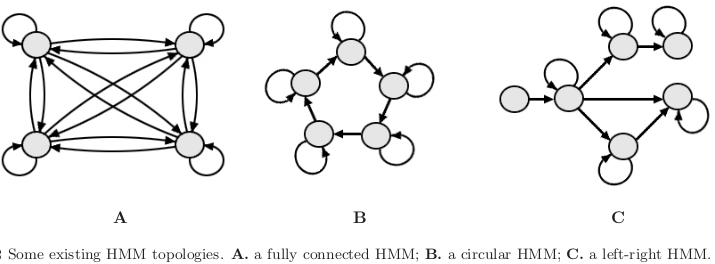
\includegraphics[width = \textwidth]{ChooHMMTopologies.png}
    \caption{Examples of the three highlighted topologies stolen from Choo.}
    \label{fig:ChooTopologies}
\end{figure}

\subsection{Hidden Markov Models} \label{Section:HiddenMarkovModels}
Yoon gives a very nice first introduction to Hidden Markov Models (HMMs): "A hidden Markov model (HMM) is a statistical model that can be used to describe the evolution of observable events that depend on internal factors, which are not directly observable." \cite{Yoon2009}. A HMM, simply put, is a model that comprises of two different parts. The first part is the sequence or the result that can be observed. A possible observed sequence could be a sequence of nucleotides or it could be a chain of events, like 20 dice throws in a row. The second part is a MC, which is \textit{hidden}, i.e. it cannot be observed. This very simple idea gives a very flexible model, which can be used for many different types of problems. The main goal is often to infer the characteristics of the hidden MC from the observed sequence. 

In a HMM, a hidden sequence of states is generated, according to the MC. This sequence will not be observable and will in (almost) all practical cases be considered as unknown. Each of the states creates, or \textit{emits}, an observed value. All these observed values are what make up the observed sequence. The emission follows a multinomial distribution, where each state follows such a distribution with different parameters. An important assumption for the HMM we will deal with is that the parameters of each multinomial only depends on the state to which it belongs \cite{Choo2004}. This means that the emitted value only depends on its respective hidden state and not on other hidden states. A HMM thus represents a doubly stochastic process: the current underlying state in the MC is stochastic, with an added layer of stochasticity in the observed value. Note that each of the hidden states should be able to produce the same symbols, i.e. the same observable values, but in different frequencies \cite{Christianini2006}.

Following the same notation as earlier, let $\mathbf{X}$ be the random vector that represents the underlying MC of length $L+1$, let $\mathcal{T}$ be the transition probability matrix, let $\mathcal{H}$ denote the hidden states, where $m = \text{card}(\mathcal{H})$, and let $\pi$ be the initial distribution of states. In addition to this, we need to define some notation for the observable sequence in the HMM. First of all, let the random vector $\mathbf{Y} = (Y_0, Y_1, \ldots, Y_L)^T$ represent an observable sequence of length $L+1$. As earlier, $\mathbf{y} = (y_0, y_1, \ldots, y_L)^T$ will represent a realization of $\mathbf{Y}$. Note that both the hidden and the observed sequence are of length $L+1$, since it is assumed that each state emits exactly one symbol. The \textit{symbol alphabet}, i.e. the set of symbols that can be emitted from each state, will be denoted by $\mathcal{S} = \{s_1, \ldots, s_M\}$, where $M = \text{card}(\mathcal{S})$. The \textit{emission probabilities}, i.e. the probabilities used in each multinomial distribution in each state, are usually arranged in a matrix as well. Denote by $\mathcal{E}$ the emission probability matrix. $\mathcal{E}$ is of dimension $m \times M$, where each row in the matrix contains the emission probabilities (of each of the symbols) for a given state. Written in mathematical terms 
\begin{align*}
    \mathcal{E}_{ij} &= \text{P}(Y_t = j|X_t = i), \hspace{0.5em} i \in \mathcal{H}, j \in \mathcal{S}.
\end{align*}
Time-homogeneity is also assumed in the stochastic process of emission, which means that these emission probabilities are the same $\forall t \in [0, L]$. 

A HMM is completely specified by $\pi$, $\mathcal{T}$ and $\mathcal{E}$, where the state space $\mathcal{H}$ and the symbol space $\mathcal{S}$ are indirectly determined by the other quantities \cite{Eddy04}. Once these quantities are specified, one can make calculations concerning the HMM. As already noted, calculating the probability of a given realization $\mathbf{x}$ is 

\begin{equation}
    \text{P}(\mathbf{X} = \mathbf{x}) = \pi(x_0)\prod_{t=2}^L\mathcal{T}_{x_{t-1}, x_t}.
    \label{ProbHiddenMC}
\end{equation}
In a similar fashion, the assumption of independence between states when generating symbols makes it possible to find the probability of the observed sequence simply by taking the product of all appropriate emission probabilities. In mathematical terms, the probability of seeing the sequence $\mathbf{y}$, given the state sequence $\mathbf{x}$, is 

\begin{equation}
    \text{P}(\mathbf{Y} = \mathbf{y}|\mathbf{X}= \mathbf{x}) = \prod_{t=1}^L\mathcal{E}_{x_t, y_t}.
    \label{ProdObservableSeq}
\end{equation}
Finally, combining these results, the joint probability of the sequences $\mathbf{x}$ and $\mathbf{y}$ is 

\begin{equation}
    \text{P}(\mathbf{X} = \mathbf{x}, \mathbf{Y}= \mathbf{y}) = \text{P}(\mathbf{X}= \mathbf{x})\text{P}(\mathbf{Y}= \mathbf{y}|\mathbf{X}= \mathbf{x}) = \pi(x_0)\mathcal{E}_{x_0, y_0}\prod_{t=2}^L\mathcal{E}_{x_t, y_t}\mathcal{T}_{x_{t-1}, x_t}.
    \label{JointProbSequences}
\end{equation}
Keep in mind that the products in equations \eqref{ProbHiddenMC}, \eqref{ProdObservableSeq} and \eqref{JointProbSequences} usually become very small in practice. This can give numerical instability when computing the probabilities. A common trick to solve this is to work with the logarithm of the probabilities. In this way, the multiplicative properties become additive, which mitigates some problems that may occur in the calculations. This is especially important when implementing the algorithms that will be discussed later \cite{Christianini2006}. 

Note that we here assume that the hidden state sequence $\mathbf{x}$ is known, which is usually not the case in practice. The state sequence needs to be inferred from the observed sequence, which is one of the main problems of a HMM, which will be explained in the following. For a more rigorous treatment of this topic, although in the topic of speech recognition, the reader is referred to \cite{Rabiner1989}.


\subsection{Basic Problems for HMMs}
http://jedlik.phy.bme.hu/~gerjanos/HMM/node6.html

As Yoon \cite{Yoon2009} and Rabiner \cite{Rabiner1989} point out in their respective articles, there are three issues that need to be resolved in order to be able to use HMMs in practical applications. In the following, these issues will be presented, together with algorithms that are used to address the problems. 

A given HMM will in the following be denoted by $\theta = (\pi, \mathcal{T}, \mathcal{E})$. This means that when we refer to a HMM $\theta$, this means that the HMM is fully specified by the three parameters and that the parameters are known. Moreover, for ease of notation, $\text{P}(\mathbf{Y} = \mathbf{y})$ will be denoted as simply $\text{P}(\mathbf{y})$ in the following. 

\subsubsection{The Evaluation Problem}
The first issue that needs to be addressed is: how can the probability $\text{P}(\mathbf{y}|\theta)$ be calculated? That is, how can one find the probability of observing the realization $\mathbf{y}$ from a given HMM $\theta$? If the exact underlying state sequence was known, this would have been easily calculated using equation \eqref{JointProbSequences}. However, the underlying state sequence cannot be observed, which means that there may exist many different underlying state sequences that can yield the same observed sequence $\mathbf{y}$. Thus, the first solution that comes to mind would be to use the law of total probability to calculate

\begin{equation}
    \text{P}(\textbf{y}|\theta) = \sum_{\forall\textbf{x}_i \in \mathcal{H}^n} \text{P}(\textbf{y}, \textbf{x}_i|\theta) = \sum_{\forall\textbf{x}_i \in \mathcal{H}^n} \text{P}(\mathbf{x}_i|\theta)\text{P}(\mathbf{y}|\mathbf{x}_i,\theta), 
\label{unfeasibleForward}
\end{equation}
where $\mathcal{H}^n$ is the space of all possible state sequences that can yield $\mathbf{y}$. Of course, $\mathcal{H}^n$ can be very large, which makes this calculation computationally infeasible. In fact, $\mathcal{H}^n$ may consist of $m^L$ sequences, since these are all the possible state sequences. Luckily, the \textit{forward algorithm} exists, which uses dynamic programming to solve this issue in a computationally feasible manner. This algorithm has time complexity $\mathcal{O}(Lm^2)$, which is a significant improvement over the exponential solution by straightforward use of equation \eqref{unfeasibleForward}. The forward algorithm is given below.  

\begin{algorithm}
    \caption{Forward Algorithm}\label{alg:Forward}
    \begin{algorithmic}
        \STATE $V \gets \text{array}((m+1) \times (L+1))$
        \FOR{$i = 0, 1, \ldots, m$}
            \STATE $V(i,0) \gets \pi(h_{i}) \mathcal{E}_{h_{i},y_0}$
        \ENDFOR
        \FOR{$i = 1, 2, \ldots, L$}
            \FOR{$j = 0,1,\ldots,m$}
                \STATE $V(j,i) \gets \mathcal{E}_{h_{j}, y_i}\sum_{k=0}^{m}V(k, i-1)\mathcal{T}_{h_{k},h_{j}} $
            \ENDFOR
        \ENDFOR
        \RETURN $\text{P}(\mathbf{y}|\theta) \gets \sum_{k=0}^{m}V(k,L)$
    \end{algorithmic} 
\end{algorithm}

Note that the forward algorithm gives a \textit{confidence measure} on the observed sequence - how confident are we that the observed sequence could have been generated by the model $\theta$. This problem is also sometimes referred to as the \textit{scoring problem}, since $\text{P}(\mathbf{y}|\theta)$ is a way to score a new observed sequence based on the given HMM \cite{Yoon2009}. If the calculated probability is lower then some "background distribution" of similar sequences, then the probability of the sequence being emitted by the HMM is low and one would conclude that the HMM is not a good model for the observed sequence. However, if the probability is high, then we can conclude that the HMM can be used in the situation. When this is verified, we tackle the \textit{decoding problem}.

\subsubsection{The Decoding Problem}
The second issue that needs to be addressed is: what state path $\mathbf{x}$ maximizes the probability of emitting the observed sequence $\mathbf{y}$, i.e. how can the \textit{optimal state path} be found? This follows the principle of maximum likelihood, which says that we should choose the hidden state path that maximizes the likelihood of yielding the observed sequence. Our best bet when trying to infer the hidden state path from the observed sequence is exactly the one that gives the maximum probability of obtaining the observed sequence. In other words, the hidden state sequence that best explains the observed sequence is the optimal state path

\begin{equation}
    \mathbf{x^*} = \argmax_\mathbf{X} \text{P}(\mathbf{X}|\mathbf{y}, \theta).
    \label{optimalStatePath}
\end{equation}
Notice that this is equivalent to finding the state sequence that maximizes $\text{P}(\mathbf{X}, \mathbf{y}|\theta)$, because of the definition of conditional probability  

\begin{equation*}
    \text{P}(\mathbf{X}|\mathbf{y}, \theta) = \frac{\text{P}(\mathbf{X}, \mathbf{y}|\theta)}{\text{P}(\mathbf{y}|\theta)}.
\end{equation*}
Again, the first solution that comes to mind would be to compare all possible state sequences $m^L$, and use equation \eqref{JointProbSequences}, but this is still computationally infeasible in most cases. Therefore, the \textit{Viterbi algorithm}, which also is based on dynamic programming, exists. The time complexity of the Viterbi algorithm is $\mathcal{O}(Lm^2)$, which is the same as for the forward algorithm. This is a large improvement over the exponential time-complexity of the straightforward solution. The Viterbi algorithm is given below. 

\begin{algorithm}
\caption{Viterbi Algorithm}\label{alg:Viterbi}
\begin{algorithmic}
    \STATE $V \gets \text{array}((m+1) \times (L+1))$
    \STATE $P \gets \text{array}((m+1) \times (L+1))$
    \FOR{$i = 0, 1, \ldots, m$}
        \STATE $V(i,0) \gets \pi(h_i) \mathcal{E}_{h_i,y_0}$
        \STATE $P(i,0) \gets -1$
    \ENDFOR
    \FOR{$i = 1, 2, \ldots, L$}
        \FOR{$j = 0,1,\ldots,m$}
            \STATE $V(j,i) \gets \mathcal{E}_{h_j, y_i}\max_{k=0,1,\ldots,m}\{V(k, i-1)\mathcal{T}_{h_k,h_j}\}$
            \STATE $P(j,i) \gets \argmax_{k=0,1,\ldots,m}\{V(k, i-1)\mathcal{T}_{h_k,h_j}\mathcal{E}_{h_j, y_i}\}$
        \ENDFOR
    \ENDFOR
    \RETURN $\text{P}(\mathbf{X}|\mathbf{y},\theta) \gets \max_{k=0,1,\ldots,m}V(k,L); \hspace{0.5em}x_L^* = \argmax_{k=0,1,\ldots,m}V(k,L)$
\end{algorithmic} 
\end{algorithm} 
Note that $\mathbf{x}^*$ is simple to find based on $x_L^*$; the optimal path $\mathbf{x}^*$ starts at $x_L^*$ and backtracks all the way to $x_0^*$ by using $P(\cdot, \cdot)$. The backtracking ends when the value $-1$ is found in $P$, i.e. when the beginning of the sequence has been reached. 

Also notice that both the forward and the Viterbi algorithms can easily be $\log$-transformed in order to gain greater numerical stability, by taking logarithms of all values and switching multiplications with additions. 

An important point to make before moving forward is that both the evaluation problem and the decoding problem are related to whether or not an observed sequence can be reasonably modeled by means of a given HMM $\theta$. But how can this model be found in the first place? This is what is often referred to as the \textit{training problem}, which will be covered next. 

\begin{comment}
\textcolor{red}{CAN write about the backward algorithm if time and if it seems relevant. }
The \textit{Backward algorithm} is an alternative ?? The backward algorithm seems like an alternative to the forward algorithm; if the largest probability is known (already found with Viterbi), then it seems like the path that correspond to this probability can be found with the backward algorithm. 

The Viterbi algorithm finds the optimal path for obtaining the entire sequence, i.e. it finds the sequence that maximizes the joint probability of obtaining the entire observed sequence. In some cases, one might be interested in finding the path that gives the largest probability of observing each symbol of the sequence individually. This can be done using the \textit{backward algorithm}. The problem here is to find the state $h_j$ that has the highest likelihood of being the hidden state of $x_j$, i.e. 

\begin{equation*}
    \hat{h}_j = \argmax_i\text{P}(h_j = i|\textbf{X}).
\end{equation*}
As before, searching all the possible states is not a viable option, which is why the backward algorithm is used. It works as ... \textcolor{red}{Continue... Reading from Yoon2009.}

But why do we care about finding the sequence of individually optimal states? This will maximize the expected number of correctly predicted states \cite{Yoon2009} \textcolor{blue}{Hvorfor det egentlig?} Well, if this is the case, why does one even bother using the Viterbi algorithm? The problem with the sequence that maximizes the probability of each observation individually is that it in general will be suboptimal, i.e. that there exists some other sequence $\mathbf{h}^*$ such that $\text{P}(\mathbf{X}, h_1h_2\ldots h_n) \leq \text{P}(\mathbf{X}, \mathbf{h}^*)$. Moreover, the sequence may not even be a possible path for the structure of the HMM, for example if some of the transitions in the predicted sequence are not possible with the given state transition probabilities of the model. For this reason, the Viterbi algorithm is preferred when our goal is to find the optimal path for the entire sequence, while the backward algorithm is preferred when our goal is to infer which state is optimal in a specific position in the sequence. Moreover, the backward algorithm can be used to conclude about the confidence of a state prediction \textcolor{red}{Continue... Reading from Yoon2009.}
\end{comment}

\subsubsection{The Training Problem}
The third issue that needs to be addressed is: how can the HMM parameters be reasonably chosen based on a set of observed sequences? For example, we have a set of sequences $\mathbf{\chi} = \{\mathbf{y}_1, \ldots, \mathbf{y}_G\}$, where each $\mathbf{y}_i, \hspace{0.2em} i \in [1,G]$ is an observed sequence of symbols, that we want to represent with a HMM. The difficulty that needs to be solved is how the parameters of the HMM can be estimated based on the set $\mathbf{\chi}$. This is what is typically called the \textit{training} or \textit{learning} problem, analogously to the need for training any other machine learning model. There exists no optimal way to train the HMM from a limited number of finite observation sequences, but there exists algorithms that can find local maximums in the observation probability. Some examples are the Baum-Welch algorithm, standard gradient based methods from optimization or simulation with Monte Carlo expectation maximization (MCEM) \cite{Yoon2009}. For detailed treatments of how the training prblem can be solved, the reader is referred to \cite{Rabiner1989}, \cite{Isaev2006} or \cite{Durbin1998}.

\subsection{HMM Variants}
There exists many variants of what we will call the standard HMM. For completeness, the standard HMM will be specified first, before the most widely used types of HMMs in bioinformatics will be presented. Note that this list is by noe means exhaustive. 

\begin{comment}
\subsubsection{Generalized HMMs}
\textcolor{red}{Changes the distribution of time until state transition (to another state) from geometric to another generalized distribution. Let's see if I have to add it here (depending on if it is used in some of the applicatins in biology. I think this is a continuous time Markov Chain (with sojourn times etc) as learned in StokMod, but not sure. } 
\end{comment}

\subsubsection{Standard HMM}
The \textit{standard HMM} is the simplest form of a HMM, which has the most restricting assumptions. In fact, the assumptions described in section \ref{Section:HiddenMarkovModels} all belong to what we will call the standard HMM. Concisely restated, the hidden MC is a discrete-state time-homogeneous first-order MC. Also, often one assumes that the MC is \textit{ergodic}, which means that every state can be reached from any other state in a finite amount of states \cite{Rabiner1989}. Moreover, each state in $\mathcal{H}$ generates exactly one output and can emit every symbol in $\mathcal{S}$. Importantly, the emitted value from each states depends only on that respective state. 

All the assumptions made in the simple model restricts the usefullness of the HMM. For example, standard HMMs do not deal well with correlations between residues, since they assume that each residue depends only on one underlying state \cite{Eddy04}. Since the Markov property is assumed, an HMM has no way of "remembering" any distant correlation between the symbols in $\mathcal{S}$. Moreover, Choo et. al writes that "the linear nature of HMM also makes it difficult to capture higher-level information or correlations among amino acids" \cite{Choo2004}. These are only some examples of how restricted the standard HMMs are. 

Despite the fact that the strong assumptions of the standard HMM restrict the flexibility of the model, one can only imagine how the assumptions can be tweaked to create a new type of HMM. Some examples of how changes in the assumptions can mitigate some om the problems of the standard HMM are shown next.  

\subsubsection{Profile-HMMs}
\textit{Profile-HMMs} (pro-HMMs) have specific architectures, which make them suitable for modeling sequence profiles \cite{Yoon2009}. Because of this, in this context, the topology of pro-HMMs are best explained with multiple sequence alignment in mind. Two simple ways to think of a pro-HMM is as an abstract description of a protein family or a statistical summary of multiple sequence alignment \cite{Christianini2006}. A pro-HMM is constructed to not contain any cycles. Moreover, a pro-HMM consists of three different types of hidden states: match states ($M_k$), insert states ($I_k$) and delete states ($D_k$). These are used to describe symbol frequencies, insertions and deletions, respectively, at each specific position in a sequence. A great example on how to build a pro-HMM, which helps to clarify the ideas, can be found in \cite{Yoon2009}. \textcolor{red}{Can I just steel this example?} The illustration from the example is shown in \ref{fig:Yoon2009ProfileHMMExample}.

\begin{figure}
    \centering
    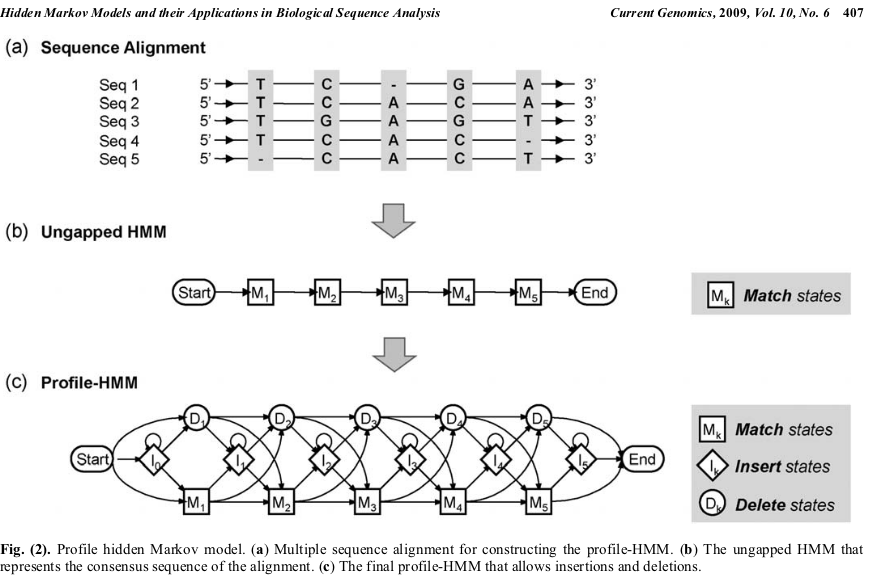
\includegraphics[width = \textwidth]{exampleProfileHMM.png}
    \caption{Example from \cite{Yoon2009}}
    \label{fig:Yoon2009ProfileHMMExample}
\end{figure}

\textcolor{red}{Kanskje dette skal flyttes til eksempelt på Multiple Sequence Alignment?}
The example shows how a profile HMM can be built from a multiple sequence alignment. The $M_k$'s are used to indicate match states, i.e. they represent the case where a symbol in the new observation matches with the state of the profile HMM. The emission probabilities from each match state are easily estimated by using the frequencies of each symbol in the match state. The ungapped HMM can represent ungapped sequences. The states $I_k$ and $D_k$ are added so that the HMM can represent sequences that contain gaps, which makes the profile HMM a much more powerful model compared to the simpler models that describe a multiple sequence alignment, like regular expressions and PSSM. It is important to note that the delete states $D_k$ are silent states; they are placeholders for missing symbols in the consensus sequence of the alignment when compared to a shorter new observed sequence. 

\subsubsection{Pair-HMMs}
In the context of bioinformatics, a \textit{pair-HMM} (p-HMM) is especially useful for finding sequence alignments and evaluating the significant of the alignments \cite{Yoon2009}. To contrast the standard HMM, a p-HMM generates an aligned pair of sequences, instead of only one sequence. An example is shown in \cite{Yoon2009} \textcolor{red}{Just steel this example as well!?} The illustration from the example is shown in \ref{fig:Yoon2009PairHMMExample}.

\begin{figure}
    \centering
    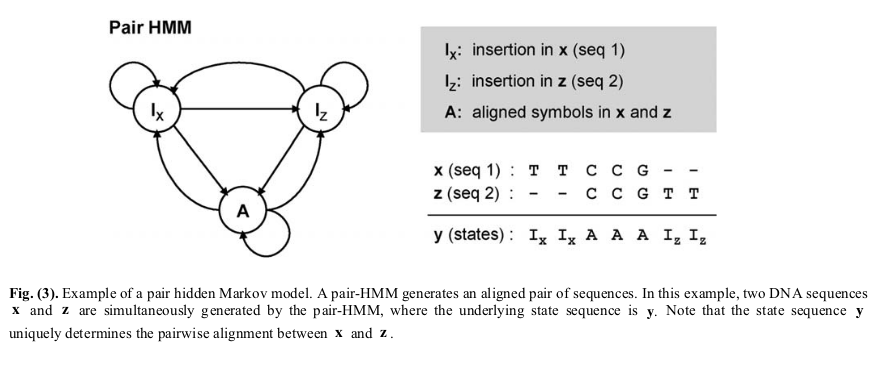
\includegraphics[width = \textwidth]{examplePairHMMYoon.png}
    \caption{Example from \cite{Yoon2009}}
    \label{fig:Yoon2009PairHMMExample}
\end{figure}

Since there is a one-to-one relationship between the hidden state sequence $\mathbf{H}$ of a pair HMM and the alignment between the two observed sequences, the alignment problem reduces to finding the optimal state path in the hidden Markov chain. This can be found by a simple variation of the Viterbi algorithm and has time complexity $\mathcal{O}(n_\mathbf{x}n_\mathbf{y})$, where $\mathbf{x}, \mathbf{y}$ are the two sequences that are aligned and $n_\mathbf{x}, n_\mathbf{y}$ are their respective lengths. The pair HMM model is an improvement over the classical sequence alignment methods, since it can be used to compute the alignment probability of the pair of sequences. A problem in the classical methods is how one should choose a punctuation scheme in order to find a biologically meaningful optimal alignment of the sequences. In cases where this is difficult to choose, it is more meaningful to compute the probability that the sequences are related, which a pair HMM makes possible \cite{Yoon2009}. This probability can be calculated by a slight modification of the forward algorithm. 

\subsubsection{Context-Sensitive HMMs}
In the context of bioinformatics, the standard HMM has limitations that make it non-suitable for dealing with RNA sequences. In order to deal with RNA sequences, one needs to extend the HMM to allow for pairwise correlations between non-adjacent symbols in the observed sequence. This is something that the ordinary HMM cannot model, since we assume that each state in the Markov chain depend only on the previous state and since each emission probability depends solely on the current state in the Markov chain. For this reason, the \textit{context-sensitive HMM}s (cs-HMMs) can be used.

The main difference between cs-MMs and the standard HMMs is that the former can use information about earlier emissions to adjust the emission probabilities at future states. This information is referred to as the "context". Thus, this makes it possible to model correlation between non-adjacent states. These HMMs use three different types of states: single-emission states ($\xi_i$),  pairwise-emission states ($\phi_i$) and context-sensitive states ($\gamma_i$). $\xi_i$ are very similar to the normal states in ordinary HMMs, since they have usual emission probabilities and do not use any additional information. $\phi_i$ have fixed emission probabilities also, but, in addition, they store the symbols that are admitted in memory. Then, when the Markov chain reaches the corresponding state $\gamma_i$, the memory is queried for the symbol that was emitted in $\phi_i$. The emitted symbol at this context-sensitive state $h_j$ is adjusted based on the retrieved symbol $h_k$. Thus, we can state the emission probability for this context-sensitive state as \textcolor{red}{Probs need to change the index notation etc here a bit. Do it after I fully understand the model!}

\begin{equation*}
    \epsilon(h_j|h_k, \gamma_i, \phi_i) = \text{P}(h_j\text{ emitted at }\gamma_i\text{ given that }h_k\text{ was emitted at }\phi_i).
\end{equation*}
Using the fact that $h_k$ is independent of $\gamma_i$ (as always is the case for emission probabilities) the join emission probability of $h_k$ and $h_j$ can be calculated

\begin{equation*}
    \text{P}(h_j, h_k|\gamma_i, \phi_i) = \text{P}(h_k|\gamma_i)\text{P}(h_j|h_k, \gamma_i, \phi_i) = \epsilon(h_k|\gamma_i)\epsilon(h_j|h_k, \gamma_i, \phi_i).
\end{equation*}
Thus, using the pair of states ($\phi_i, \gamma_i$) pairwise symbol correlation can be modeled for any pair by specifying these emission probabilities. A simple example of a csHMM is shown in \cite{Yoon2009} \textcolor{red}{Kan jeg bare stjele dette eksempelet også!?}. 

\begin{figure}
    \centering
    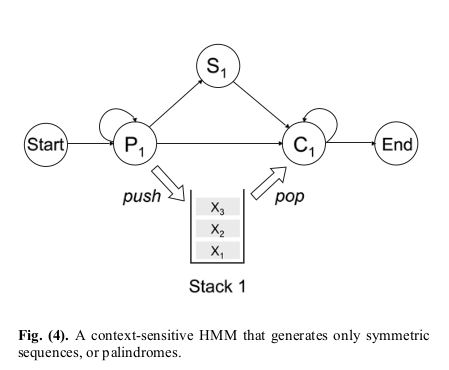
\includegraphics[width = \textwidth]{ExampleYooncsHMM.png}
    \caption{Example from \cite{Yoon2009}. I should make a similar example, but for repeating sequences instead of for palindromes, as Yoon did. This would be almost the same, but the result is slightly different.}
    \label{fig:Yoon2009ContextSensitiveHMMExample}
\end{figure}

An example of a profile csHMM is shown in \cite{Yoon2009} \textcolor{red}{Kan jeg bare stjele dette eksempelet også!?}

\begin{figure}
    \centering
    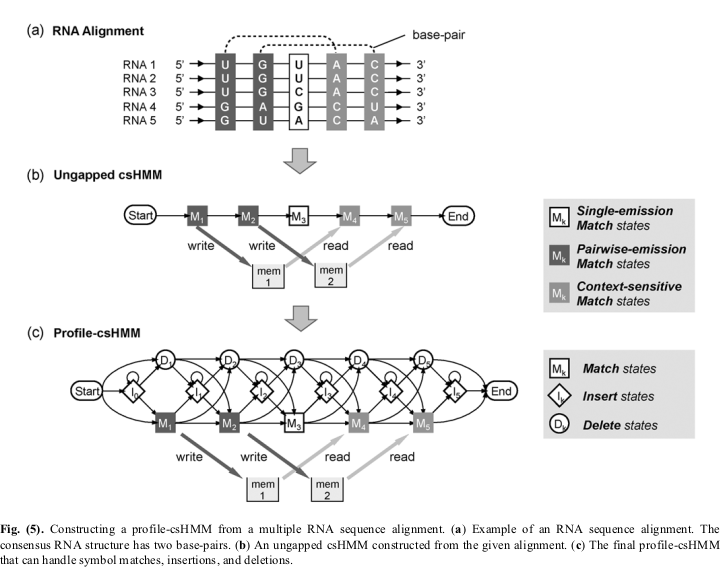
\includegraphics[width = \textwidth]{contextSensHMMExampleYoon.png}
    \caption{Example from \cite{Yoon2009}. \textcolor{red}{Tenker at jeg stjeler dette eksempelet, da det er veldig godt (eller bare henviser), men lager de to andre litt selv etter hvert!}}
    \label{fig:Yoon2009ProfileContextSensitiveHMMExample}
\end{figure}

Remember that profile HMMs were used to make profiles that represent multiple alignments of sequences, which in the context of biology can be DNA or proteins (sequences of aminoacids). Imagine that we want to make profiles that take column-wise correlations in the multiple alignment into account. This can be done relatively easily by combining the ideas of the profile HMM and the csHMM, into what we call a profile csHMM. Like for the profile HMMs studied earlier, the profile csHMMs contain match states ($M_k$), insert states ($I_k$) and delete states ($D_k$). The difference is that the match states can be of three different types, to account for symbols that are pairwise correlated. As expected, this model has the match states single-emission match states ($\xi_{m,i}$),  pairwise-emission match states ($\phi_{m,i}$) and context-sensitive match states ($\gamma_{m,i}$). The single-emission match states are used to represent columns in the multiple alignment that are uncorrelated with the others, while the pairing of ($\phi_{m,i}, \gamma_{m,i}$) are used to model pairwise correlation between symbols in different columns. An example, taken from \cite{Yoon2009}, is shown in figure \ref{fig:Yoon2009ProfileContextSensitiveHMMExample}.

\section{Applications in Bioinformatics}
Some more applications listed on the Wikipedia page: 
%https://en.wikipedia.org/wiki/Hidden_Markov_model#Applications

\subsection{Pairwise Sequence Alignment}
Pairwise sequence alignment is done to infer functional, structural and/or evolutionary relationships between two sequences. Such an alignment can be done both locally and globally and there exists a variety of methods of doing it. Optimal algorithms exist, such as the Needleman-Wunsch algorithm for optimal global alignment and the Smith-Waterman algorithm for optimal local alignment. These algorithms are based on dynamic programming and can be time consuming to use. Therefore, algorithms based on heuristics were developed, where the two most popular algorithms are called BLAST and FASTA. \textcolor{red}{Proteins or DNA? Only proteins? Sjekk for alle algoritmene her!} All the mentioned algorithms work well for highly similar sequences, but produce mediocre results for highly divergent sequences \cite{Choo2004}. Profile based analysis was developed to improve these results, in which HMMs play a crucial role. 

p-HMMs can be used when tackling the pairwise sequence alignment problem as a stochastic process, as used by Smith et al \cite{Smith2003} \textcolor{red}{Skumles artikkelen og sjekk at det faktisk stemmer!} Pairwise sequence alignment is the typical example of use of a p-HMM in bioinformatics, as also mentioned in the theoretical part concerning the model. \textcolor{red}{Complete this after completing theory about p-HMMs, because I think it will be easier then!}

Goal: Infer functional similarity \textcolor{red}{Could be merged with "Prediction of Function" perhaps?}. Can use a Pair HMM \cite{Choo2004} (go to source after Choo). 

As noted, p-HMMs are a great alternative to using classical sequence alignment techniques and evaluating the statistical significance of the alignment. 

Pair Hidden Markov models on tree structures (PHHMTS) can be used for aligning trees. Since most RNA secondary structures can be represented as trees, this provides a useful framework for aligning RNA sequences. 

\subsection{Multiple Sequence Alignment}
Multiple sequence alignment is commonly used to find conserved regions in a group of sequences and/or predicting protein structures. In contrast to the pairwise sequence alignment problem, there does not exist any optimal algorithms to solve the multiple alignment problem. However, there exists a variety of heuristic methods for solving it. One possible solution is to reduce the multiple alignment problem down to a set of pairwise comparisons between the sequences, in an orderly fashion, in order to end up with the multiple alignment in the end. Here one can choose to use either the optimal algorithms or the heuristic algorithms when performing the pairwise alignment. One type of methods that employs this paradigm is referred to as progressive sequence alignment. More details on a progressive algorithm that uses Needleman-Wunsch for the pairwise alignment can be found in \cite{Feng1987}. Some commonly available implementations of this solution include the T-Coffee and the Clustal package \cite{EMBL-EBI-Multiple}. Another type of methods that uses this paradigm is referred to as iterative alignment. These methods are slightly different than the progressive methods, since they allow realignment of the pairwise sequences during multiple iterations, where the progressive methods depends highly on the initial pairwise alignment of the first two sequences \cite{BioInfoOrgMSA}. One popular openly available implementation of an iterative method is MUSCLE \cite{EMBL-EBI-Multiple}. 

As in the case of pairwise alignment, HMMs provide powerful alternatives to these other methods for multiple alignment. In this problem, pro-HMMs have been particularly successful \cite{Choo2004}. \textcolor{red}{Continuing to read in Choo.}

Pro-HMMs have been applied to this problem with much success. Is connected to the Viterbi algorithm also.   

\textcolor{red}{Må virkelig få strukturert dette skikkelig! Vanskelig å dele opp alt slik jeg tenkte opprinnelig! Mulig jeg bør samkjøre teori og applications i større grad, selv om jeg egentlig ville ha dem separert!}

\verb$http://pfam.xfam.org/$

Pro-HMMs are defined in order to solve the problem of multiple alignment of sequences. All new sequences can efficiently be aligned against this pro-HMM. They also facilitate quick assignment of protein function. These pro-HMMs are commonly regarded as a summary of a multiple alignment of sequences or as a model for a family of such sequences \cite{Christianini2006}. 

Since pro-HHMs are an abstract representation of a multiple alignments, they can be used to produce pairwise or multiple alignments as well. Thus, aligning a sequence with a pro-HHM is equivalent to aligning the sequence to many, many other sequences, which where used to establish the pro-HMM in the first place \cite{Christianini2006}. E.g. PFAM is a free online repository, that store pro-HMMs of many known protein families. PROSITE is another database that stores pro-HMMs. 

The pro-HMMs are very useful in the context of searching for homologues. Given a pro-HMM that represents a family of sequences, one can use this model to search in a database of sequences, in order to find additional homologues to the family. Similary, given a database of pre-built pro-HMMs (like PROSITE or PFAM), we can look for matching profiles to a symbol sequence. Thus, we can use this database to classify and annotate the given sequence. 

Pro-HMMs can also be used to compare two different multiple sequence alignments (sequence profiles). This can be beneficial for detecting remote homologues \cite{Yoon2009}. "These profile HMMs are also what makes it possible to assign protein function quickly, and can be regarded both as a summary of a multiple alignment and as a model for a family of sequences" \cite{Christianini2006}.

Many multiple sequence alignment algorithms also use p-HMMs \cite{Yoon2009}. The most widely used approach based on p-HMMs is called progressive alignment. 

\subsection{Motif Representation (or Identification?)}
A motif is a recurring pattern in DNA or proteins, which is assumed to be related to biological function. Thus a motif can be a sequence of nucleotides or of amino-acids. Finding such motifs is interesting to a biologist because \textit{transcription factor binding sites} (TFBS) appear as such motifs in sequences. These are regulatory sequences that control gene transcription, which is important information for a biologist because they repress or promote the expression of many other genes \cite{Christianini2006}.

There are several ways of representing such sequence motifs, where the performance of each method generally depends on what type of motifs one wants to represent. For shorter, ungapped motifs of fixed length, methods like \textit{consensus sequences}, \textit{regular expressions} (RegEx), \textit{sequence logos} and \textit{position specific scoring matrix} (PSSM), in ascending order of complexity, are commonly used. Note that these can also be seen as different ways of visualizing or representing multiple sequence alignments, which are useful tools in practice, since the alignments themselves are not very easy in use. 

The drawbacks of these methods are that they do not work well for longer motifs with variable length gaps. This is where the profile-HMMs shine in comparison. The HMMs work well for all types of motifs, including the short and fixed length motifs, but they are more complicated models. Thus, even though the HMMs always will produce good results, given that they can be built correctly in the specific case, one should not always use these models because of their complexity. Always keep the principle of parsimony in mind; for competing explanations, or models, where all are reasonable, one should always choose the simplest, with the least amount of assumptions. Hence, even though the HMMs are great tools also for motif identification, they should be used when appropriate. 

But how can the HMMs be used to represent motifs with variable length gaps? The profile-HMMs have gained much traction for this problem, since it yields very reliable results. How they work can be seen easily from the example presented about the profile-HMMs in the section on theoretical background, since the example talks about how to represent a multiple sequence alignment as a profile-HMM. The same principle explained in the example can be used when working with much larger and more complicated alignments. 

After constructing these representations, they can be used to search for sequences that belong to the same family as the aligned sequences, since sequences that have the same motifs may share the same functions. \textcolor{red}{Good idea to have this as a different section compared to the multiple sequence alignment-section?}

Note that the problem of finding the motifs is not discussed in detail here, as this is a much more complicated problem compared to simply representing the motifs. However, this problem is highly similar to multiple local alignment, which has been explained in detail earlier. An example of such an algorithm is given in chapter 10.3 in \cite{Christianini2006}, which is a variant of the Gibbs sampling algorithm based on PSSMs. 

EXTRA, if needed: 
Wikipedia: When a motif appears in the exon of a gene, it can encode a "structural motif" of a protein. Outside of gene exons, there exists regulatory sequence motifs 

\subsection{Prediction of Function}
HMMs are used to make probabilistic statements about the function of proteins and thus, they can also be used to assign proteins to families of unknown function \cite{Christianini2006}. \textcolor{red}{Is this a step in Genome Annotation? Perhaps they should be merged then! Or multiple sequence alignment?}

\subsection{Segmentation}
Segmentation is about defining exact boundaries between distinct regions with different chemical properties. Moreover, segmentation is about defining larger sequences of heterogeneous nucleotide in genome and to identify biological features that are responsible for the heterogeneity that is observed \cite{Christianini2006}. Some classical methods are ...

HMMs can be used effectively for segmentation as well... They can help to define regions of gene and protein sequences with various chemical properties \cite{Christianini2006}. 

Example 4.2 in \cite{Christianini2006} shows an example of segmentation using HMMs.

In the setting of segmentation, the hidden states are interpreted as different types of the sequence and the hidden alphabet is typically very small. The underlying MC is cyclic in this case, allowing returns to the same state, i.e. to the same type of sequence, many times during the simulation \cite{Christianini2006}. 

\subsection{Protein Homology Detection}
Goal: Determine which proteins are derived from a common ancestor. 

\textcolor{red}{Not sure if the following fits in here.}
Characterize sets of homologous proteins (gene families) based on common patterns in their sequence. This allows us to determine if a new protein belongs to a certain family or not \cite{Christianini2006}. In thi case HMMs can be used to provide a more flexible characterization of sequence patterns. This, in comparison to the simpler way of using multiple alignment to construct a PSSM, also works well for cases which include gaps of variable length, which is a case where the multiple alignment method does not work well \cite{Christianini2006}. This type of homology detection is done with profile HMMs. "profile HMMs encode position-specific information about
the frequency of particular amino acids as well as the frequency of insertions
and deletions in the alignment. They are constructed from multiple alignments
of homologous sequences" \cite{Christianini2006}. Since pHHMs are an abstract representation of a multiple alignments, they can be used to produce pairwise or multiple alignments as well. Thus, aligning a sequence with a pHHM is equivalent to aligning the sequence to many, many other sequences, which where used to establish the pHMM in the first place. 

Feature-based Profile HMMs can be used to improve the performance of remote protein homology detection \cite{Yoon2009}.

\textcolor{red}{This is just an application of multiple sequence alignment, no? So perhaps those two can be merged?}


\subsection{Gene Prediction / Genomic Annotation (?) / Gene Finding (?)}
\textcolor{red}{Is Gene Prediction and Genomic Annotation (and Gene Finding) the same problem? Two different words for the same name or are they slightly different problems, with different goals in mind?}

HMMs are employed to find eukaryotic genes and to find pseudogenes, which look like functioning genes except for some misplaced stop codons. They are very useful for these problems because of their flexibility \cite{Christianini2006}.

If the hidden states in the HMM can be inferred, the genome can be better annotated or one can understand the dynamics of the genome better \cite{Christianini2006}.

Genomic annotation: Generalized HMMs \cite{Choo2004}.

Eukaryotic genes can be modeled using HMMs \cite{Yoon2009}. 

Pair HMMs can be used for gene prediction \cite{Yoon2009}.


\subsection{Protein Sequence Classification}

Profile HMMs (analagously to multiple sequence alignment). 


\subsection{Protein Structure Prediction}
Is connected to homology detection. More in \cite{Choo2004}.

Profile HMMs can be used to "model sequences of protein secondary structure symbols: helix (H), strand (E) and coil (C)" \cite{Yoon2009}. This model can be used to recognize the three-dimensional fold of new protein sequences based on their secondary protein structure predictions. 

Also page 79 in Introduction to Mathematical Methods in Bioinformatics. 


\subsection{Base-calling}
\cite{Yoon2009}
\subsection{Modeling DNA Sequencing Errors}
\cite{Yoon2009}
\subsection{ncRNA Identification}
\cite{Yoon2009}
\subsection{RNA Structural Alignment}
As explained when talking about context-censitive HMMs (csHMMs), profile-csHMMs can be used to perform structural alignment of RNA and performing similarity searches, analagously to how the profile-HMMs can be used to perform multiple alignment of DNA or proteins and performing similarity searches in these cases. RNA sequence analysis is often of high computational complexity, because the alignment algorithms have to deal with base-pair correlations in the sequences that may be very complicated. More about this problem in \cite{Yoon2009}.

\section{Examples in R}

\subsection{CG-islands and the "Fair Bet Casino"}

"An introduction to bioinformatics algorithms" - Jones and Pevzner Page 388. 

Hay una tarea sobre esto tambien, descargado en pdf en "Books/bioinfo".

\textcolor{red}{The reference list should be alphabetically ordered later!}
\begin{thebibliography}{20}
\bibitem{Eddy04}
Sean R. Eddy (2004) \emph{What is a hidden Markov model?}, Nature Biotechnology, Volume 22, Number 10, 1315-1316.

\bibitem{Choo2004} 
Khar H. Choo, Joo C. Tong, Louxin Zhang (2004) \emph{Recent Applications of Hidden Markov Models in Computational Biology}, Geno. Prot. Bioinfo, Vol. 2, No. 2, 84-96.

\bibitem{Yoon2009}
Byung-Jun Yoon (2009) \emph{Hidden Markov Models and their Applications in Biological Sequence Analysis}, Bentham Science Publishers Ltd., Current Genomics, Vol. 10, No. 6, 402-415.

\bibitem{Christianini2006}
Nello Christianini, Matthew W. Hahn (2006) \emph{Introduction to Computational Genomics: A Case Studies Approach}, Cambridge University Press.

\bibitem{Smith2003}
Smith, L., et al. (2003) \emph{Hidden Markov models and op-
timized sequence alignments}, Computational Biology and Chemistry, Vol. 27, 77-84.

\bibitem{Feng1987}
Feng DF, Doolittle RF (1987) \emph{Progressive sequence alignment as a prerequisite to correct phylogenetic trees}, J Mol Evol. Vol. 25, No. 4, 351-360. doi: 10.1007/BF02603120. PMID: 3118049.

\bibitem{Pinsky2011}
Mark A. Pinsky, Samuel Karlin (2011) \emph{An Introduction to Stochastic Modeling}, Fourth Edition, Elsevier

\bibitem{EMBL-EBI-Multiple}
%https://www.ebi.ac.uk/Tools/msa/ 
DENNE MÅ FØRES OPP ORDENTLIG!

\bibitem{BioInfoOrgMSA}
%https://www.bioinformatics.org/wiki/Multiple_sequence_alignment
DENNE MÅ FØRES OPP ORDENTLIG!

\bibitem{Rabiner1989}
Lawrence R. Rabiner (1989) \emph{A tutorial on hidden Markov models and selected applications in speech recognition}, Proceedings of the IEEE, Vol. 77, No. 2, 257-286

\bibitem{Isaev2006}
Alexander Isaev (2006) \emph{Introduction to Mathematical Methods in Bioinformatics}, Springer-Verlag

\bibitem{Durbin1998}
R. Durbin, S. Eddy, A. Krogh, G. Mitchison (1998) \emph{Biological Sequence Analysis}, Cambridge University Press

\end{thebibliography}

\end{document}
